\documentclass[11pt, aspectratio=169]{beamer}

% English setup
\usepackage[english]{babel}
\usepackage{booktabs}
\usepackage{tikz}
\usepackage{graphicx}
\usepackage{listings}
\lstset{
  basicstyle=\ttfamily\scriptsize,
  frame=single,
  breaklines=true,
  numbers=left,
  numberstyle=\tiny
}

% Theme settings
\usetheme{Madrid}
\usecolortheme{orchid}

% Visualization settings
\AtBeginSection[]{
  \begin{frame}
    \vfill
    \centering
    \begin{beamercolorbox}[sep=8pt,center,shadow=true,rounded=true]{title}
      \usebeamerfont{title}\insertsectionhead\par%
    \end{beamercolorbox}
    \vfill
  \end{frame}
}

\AtBeginSubsection[]{
  \begin{frame}{\insertsectionhead}
    \tableofcontents[currentsection, currentsubsection, subsectionstyle=show/shaded/hide]
  \end{frame}
}

% Title information
\title{Mathematical Analysis of Jamming and Simulation Environment}
\subtitle{Communication Jamming}
\author{Student ID: 1280391 \\ Natsuka Hosokawa}
\institute{Kochi University of Technology}
\date{\today}

\begin{document}

\begin{frame}
  \titlepage
\end{frame}

\begin{frame}{Table of Contents}
  \tableofcontents
\end{frame}

% --- Content ---

\begin{frame}{Progress}
  \begin{enumerate}
    \item Communication Jamming in SAGIN
    \item Overview of SAGIN
    \item Communication Jamming Overview
    \item Mathematical Analysis (Current Focus)
  \end{enumerate}
\end{frame}

\section{Mathematical Analysis of Jamming}
\subsection{Prerequisites}

\begin{frame}{Prerequisites}
  \begin{itemize}
    \item \textbf{Likelihood Function} $f(y|s)$ \\
      Represents how plausible a transmitted signal $s$ is, given a received signal $y$.
    \item \textbf{Characteristic Function} \\
      Transforms a linear sum of variables into a product of exponentials, simplifying statistical analysis.
    \item \textbf{Q-function} $Q(x)$ \\
      The integral of the standard normal distribution from $x$ to $\infty$.
    \item \textbf{BPSK} \\
      A digital modulation scheme: recognizes $1$ as amplitude $A$ and $0$ as $-A$.
  \end{itemize}
\end{frame}

\subsection{Signal Detection}

\begin{frame}{Maximum Likelihood Detection (MLD)}
  Assuming all symbols $s \in S$ have equal prior probabilities, we maximize the likelihood function $f(y|s)$:
  \begin{align*}
    \hat{s} = \arg \min \limits_{s \in S} |y - s|^2
  \end{align*}
  This reduces to minimizing the Euclidean distance in the signal space. Although expressed mathematically, it is essentially a simple decision of which symbol, $1$ or $0$, is closer to the received value.
\end{frame}

\subsection{Noise Aggregation}

\begin{frame}{Noise Modeling}
  The system includes natural AWGN ($w$) and jamming noise ($z$). The received signal $y$ is defined as:
  \begin{align*}
    y = s + w + z
  \end{align*}
  Using the characteristic function, the total noise can be modeled as a combined Gaussian distribution: $\mathcal{N}(0, \sigma_w^2 + \sigma_z^2)$.
\end{frame}

\subsection{Impact of Jamming}

\begin{frame}{Information Loss (1)}
  Analyzing the limit as jamming power approaches infinity ($\sigma_z^2 \rightarrow \infty$):
  \begin{align*}
    \lim \limits_{\sigma_z^2 \rightarrow \infty} P_e &= \lim \limits_{\sigma_z^2 \rightarrow \infty} Q \left( \frac{A}{\sqrt{\sigma_w^2 + \sigma_z^2}} \right) \\
    &= Q(0) = \frac{1}{2}
  \end{align*}
  The bit error rate converges to $0.5$, indicating a total loss of information.
\end{frame}

\begin{frame}{Information Loss (2)}
  From the Shannon-Hartley theorem:
  \begin{align*}
    C &= \lim \limits_{\sigma_z^2 \rightarrow \infty} B \log_2 \left(1 + \frac{A^2}{\sigma_w^2 + \sigma_z^2} \right) \\
    &= B \log_2(1) = 0
  \end{align*}
  The channel capacity vanishes.
\end{frame}

\begin{frame}{Visualizing Jamming Effect}
  \begin{figure}[htpb]
    \centering
    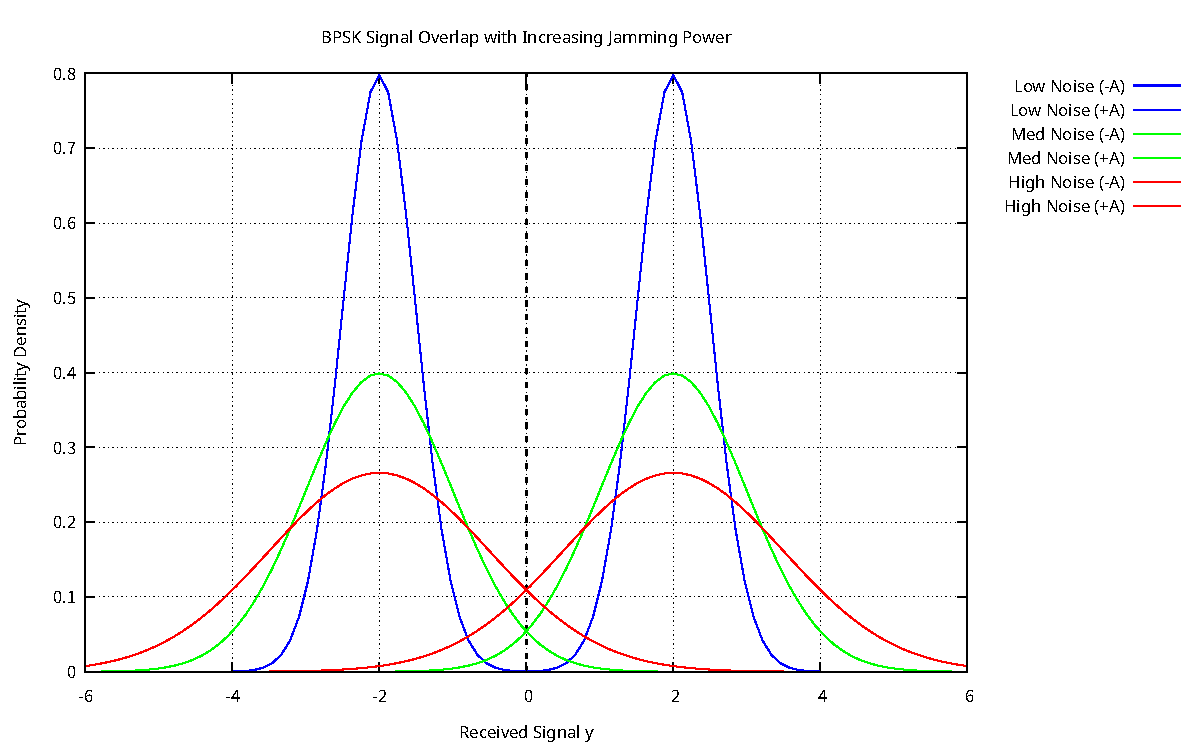
\includegraphics[width=9cm]{jamming_merged.pdf}
    \caption{BPSK Signal Overlap under Jamming}
  \end{figure}
\end{frame}

\subsection{Summary}

\begin{frame}{Summary}
  \begin{block}{Jamming Power Dependency}
    The analysis shows that the communication reliability is heavily dependent on the jamming noise intensity. Higher jamming power severely degrades communication quality, ultimately leading to a random guess state.
  \end{block}
\end{frame}

\section{Environment Setup}

\begin{frame}{Environment Setup}
  Deployed \texttt{Pyjama} on the \texttt{shikharlab-01} server.
  \begin{itemize}
    \item Directory: \texttt{jamming\_env} (under home)
    \item Files: \texttt{Dockerfile}, \texttt{docker-compose.yml}
    \item Access: SSH to server, then Terminal or VS Code for container access.
    \item Recommendation: VS Code (best for Jupyter environment).
    \item Access: Port \texttt{8080} exposed on the server.
    \item Note: Performance may differ due to the remote environment.
  \end{itemize}
\end{frame}

\section{Future Plan}

\begin{frame}{Future Plan}
  \begin{itemize}
    \item Study Reinforcement Learning (RL) in Dr. Wei's seminar.
    \item Study Game Theory to apply to anti-jamming strategies and prediction.
    \item Develop a Python program for basic jamming simulation.
  \end{itemize}
\end{frame}

\section{References}
\begin{frame}[allowframebreaks]{References}
  \begin{thebibliography}{9}
    \setbeamertemplate{bibliography item}[book]
    \bibitem{shannon}
      C. E. Shannon, "A Mathematical Theory of Communication," 
      \textit{Bell System Technical Journal}, 1948.
    \setbeamertemplate{bibliography item}[article]
    \bibitem{survey}
      H. Zeng et al., "Jamming Attacks and Anti-Jamming Strategies in Wireless Networks: A Comprehensive Survey," 
      \textit{IEEE Communications Surveys \& Tutorials}, 2024.
    \bibitem{sagin}
      K. Yang et al., "Communications in Space–Air–Ground Integrated Networks: An Overview," 
      \textit{Space: Science \& Technology}, 2025.
  \end{thebibliography}
\end{frame}

\end{document}